\chapter{Img-spy}
\label{S:img-spy}

As seen in the introduction, the main objective of this project is to develop
an open-source cross-platform software with a user-friendly interface. For this
purpose, \textbf{Img-spy was created}. The overall concept of the application
is to give some well-defined tools to be used in a digital forensics analysis. 

\section{Application walk around}

The first time the application is launched, a window asking to select a case
appears (Figure \ref{F:img-spy-select-case}). That means to select a folder of
user's local computer. If it was used before, all previous progress will be 
recovered.

\begin{figure}[htb]
	\begin{center}
		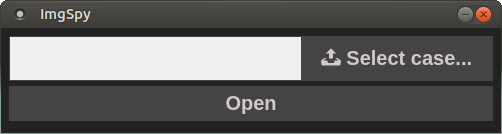
\includegraphics[width=0.7\textwidth]{./figures/img-spy-select-case.png}
		\caption{Img-spy case selector}
		\label{F:img-spy-select-case}
	\end{center}
\end{figure}

Once the case to work is picked, the main application window (Figure
\ref{F:img-spy-case-window}) is shown. This one contains tree tools needed to
proceed with the analysis. Each tool is represented with an icon.

\begin{figure}[htb]
	\begin{center}
		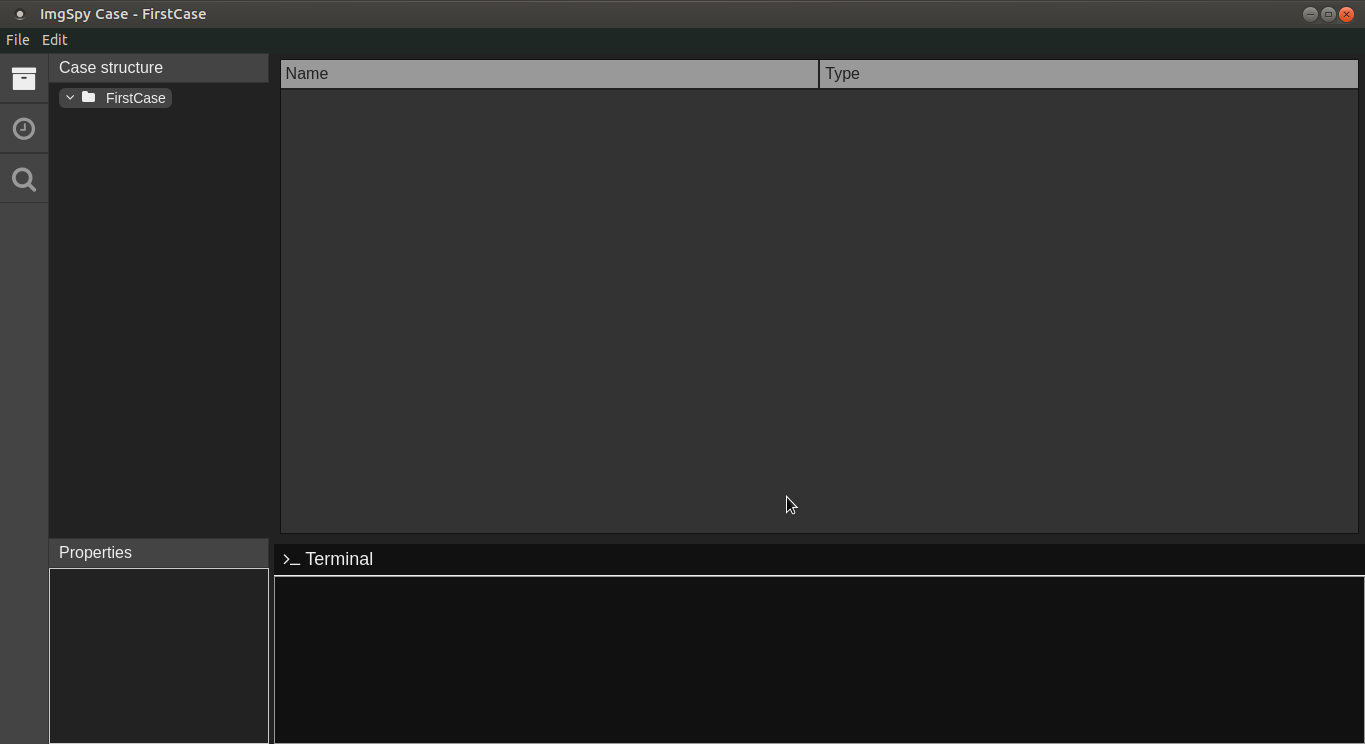
\includegraphics[width=0.7\textwidth]{./figures/img-spy-dark.png}
		\caption{Img-spy case window}
		\label{F:img-spy-case-window}
	\end{center}
\end{figure}


\begin{itemize}
	\item[] \icon{./figures/icon-dark-explorer.png}{Explorer}
	It examines images in a non-intrusive way.

	\item[] \icon{./figures/icon-dark-timeline.png}{Timeline}
	It generates a list with the activity on the file system.

	\item[] \icon{./figures/icon-dark-search.png}{Search}
	It searches a string inside an image.

\end{itemize}

One objective of the project was to be a user-friendly user interface. Many
people find inconvenient to work many hours with a bright screen while others
prefer to have more light in order to see things clearly. For that reason
multiple themes are supported. (Figure \ref{F:img-spy-multi-theme}). 

\begin{figure}[htb]
	\begin{center}
		\begin{subfigmatrix}{2}
			\subfigure[Dark theme]
			{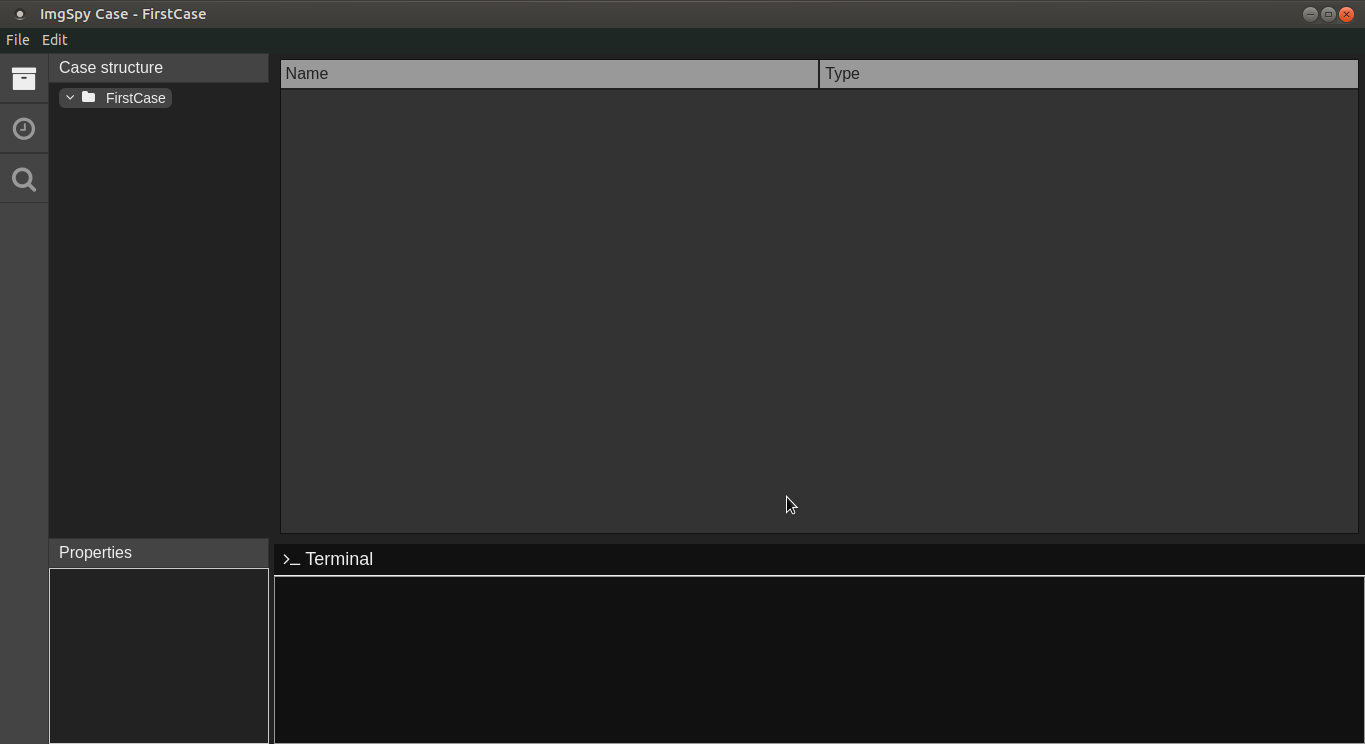
\includegraphics{./figures/img-spy-dark.png}\label{SF:S1}} 
			\subfigure[Light theme]
			{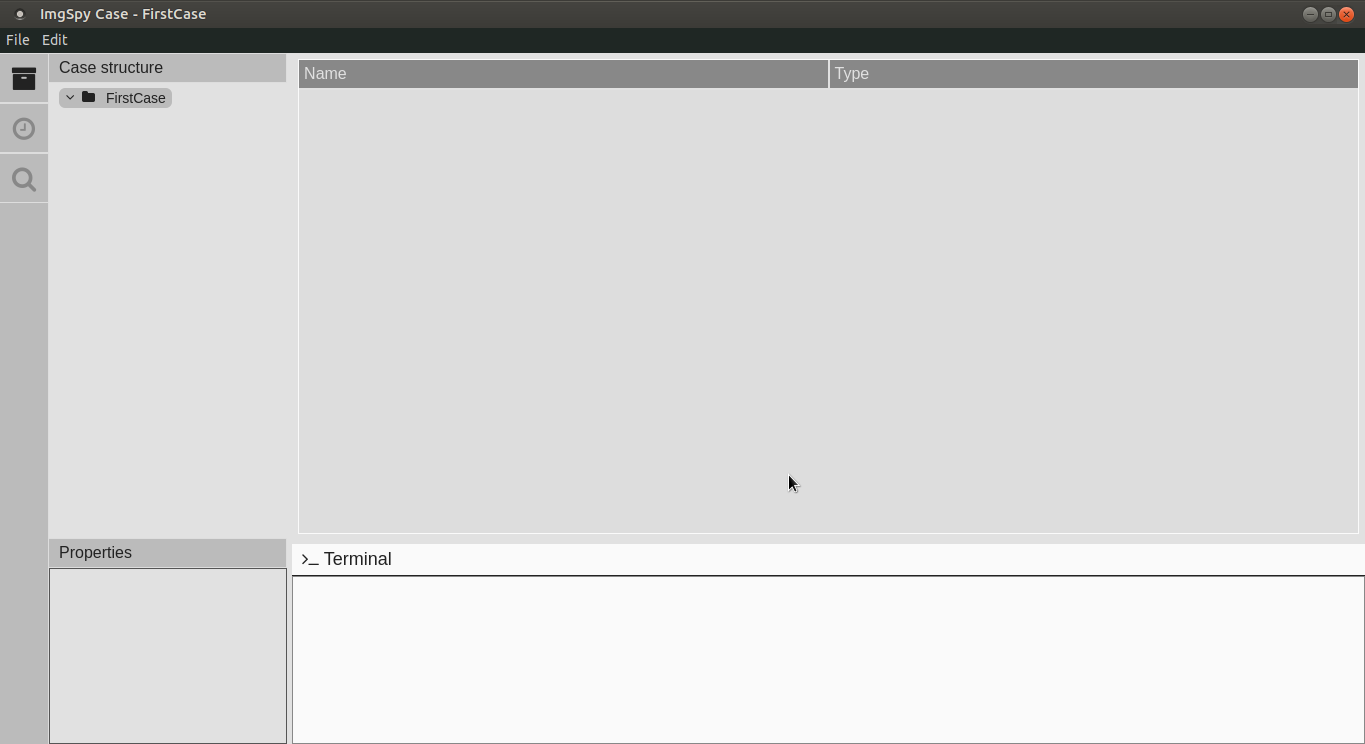
\includegraphics{./figures/img-spy-light.png}\label{SF:S1}}
		\end{subfigmatrix}
		\caption{Img-spy  multiple themes support}
		\label{F:img-spy-multi-theme}
	\end{center}
\end{figure}

\subsection{Explorer}

As seen before, \textit{Explorer} examines images in a non-intrusive way. To do
that, tsk-js analyze, list and get functions are used. Its layout contains four
panels: case structure, properties, active item content and terminal. The size
of all panels can be changed to let user feel more comfortable with the 
interface.

\subsubsection{Case structure}
\label{S:case-structure}

All folders inside the selected case folder are shown using a tree in this 
panel (Figure \ref{F:img-spy-explorer-case-structure}).

\begin{wrapfigure}[18]{L}{4.9cm}
	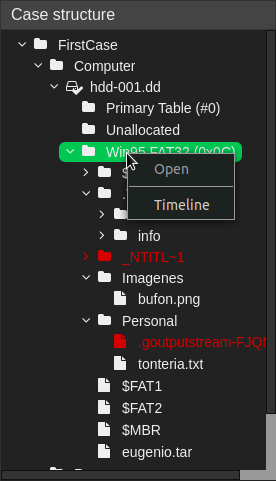
\includegraphics[width=4.4cm]{./figures/explorer-case-structure.png}
	\centering
	\caption{Explorer case structure panel}
	\label{F:img-spy-explorer-case-structure}
\end{wrapfigure}

The \textit{Explorer} is always watching case folder file system and each
change is detected launching an action to updates the application global state
refreshing the case structure tree. 

If one file have the extension \textit{.dd}, function tsk-js analysis is
executed in parallel and the image digest is computed. Once the proper hash is
provided on the image properties panel (Chapter \ref{S:explorer-properties}),
the content inside the image is added into the case tree using tsk-js list
function. Items in red color are deleted.

Each item tree have a context menu. All files can be opened with the OS
preferred applications with the open option.

Folders inside an image also have an option to generate a timeline. In case of
a disk image, partitions are treated as directories.

Finally, files have an option to export its content using tsk-js get function.

\subsubsection{Properties}
\label{S:explorer-properties}

\begin{wrapfigure}[10]{R}{6cm}
	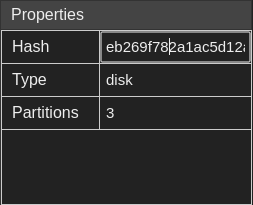
\includegraphics[width=5.5cm]{./figures/explorer-properties.png}
	\centering
	\caption{Img-spy explorer properties}
	\label{F:img-spy-explorer-properties}
\end{wrapfigure}

This panel (Figure \ref{F:img-spy-explorer-properties}) shows the properties of
the item selected on case structure (Chapter \ref{S:case-structure}).
Image properties are:

\begin{description}
	\item[Hash] This is the only editable field. Is the expected digest of the 
	image. 

	\item[Type] This value is retrieved from the tsk-js analysis. Can be disk
	or partition.
	
	\item[Partitions] If type is disk, it shows up the number of partitions
\end{description}

\subsubsection{Active item}

It displays the information of current selected item on case structure (Chapter
\ref{S:case-structure}).

\begin{figure}[htb]
	\begin{center}
		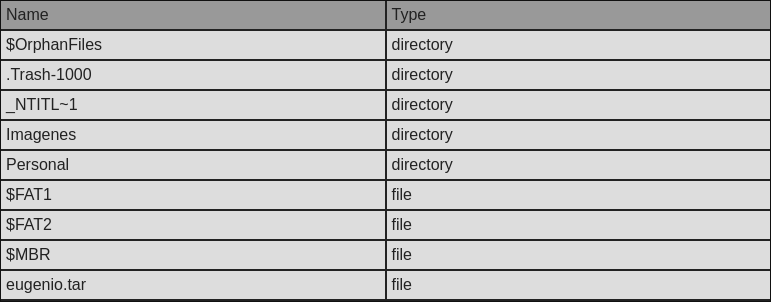
\includegraphics[width=0.7\textwidth]
		{./figures/explorer-active-folder.png}
		\caption{Img-spy active panel with a folder selected}
		\label{F:img-spy-active-folder}
	\end{center}
\end{figure}

On the one hand, when a folder is selected, active panel shows the files inside
it (Figure \ref{F:img-spy-active-folder}). If the user clicks one row, the
current active item will be the clicked one, updating also the case structure
(Chapter \ref{S:case-structure}).

\patchcmd{\subfigmatrix}{\hfill}{\hspace{0.2cm}}{}{}
\begin{figure}[htb]
	\begin{center}
		\begin{subfigmatrix}{2}
			\subfigure[Hexadecimal view]
			{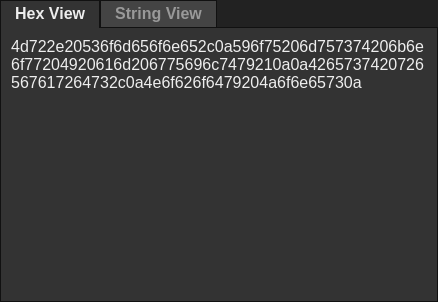
\includegraphics[width=0.4\textwidth]
			{./figures/explorer-active-file-hex.png}} 
			\subfigure[String view]
			{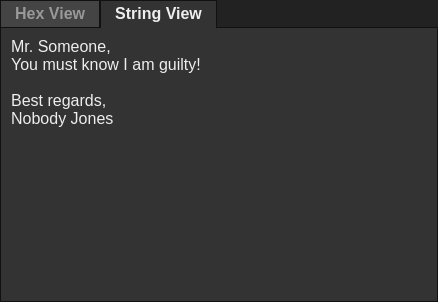
\includegraphics[width=0.4\textwidth]
			{./figures/explorer-active-file-string.png}}
		\end{subfigmatrix}
		\caption{Img-spy active panel with a file selected}
		\label{F:img-spy-active-file}
	\end{center}
\end{figure}

On the other hand, Figure \ref{F:img-spy-active-folder} shows the active panel
when a file is selected. Since the content type of the files is not known,
two type of views are supported: hexadecimal and string. It only displays
the first thousand characters to not freeze the user interface. A future line
of the project is to implement a view more functionality.

\subsubsection{Terminal}

There are many asynchronous tasks that keep some time to be executed, for 
instance, tsk-js analysis. The terminal logs those tasks and possible outputs.
Figure \ref{F:img-spy-explorer-terminal} shows some logs.


\begin{figure}[htb]
	\begin{center}
		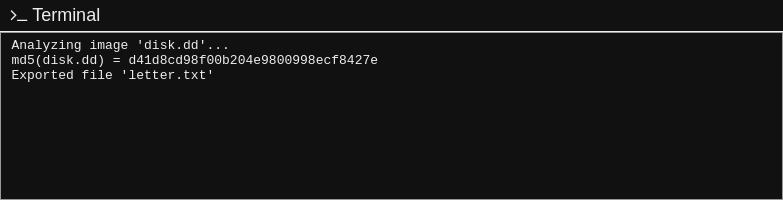
\includegraphics[width=0.9\textwidth]
		{./figures/explorer-terminal.png}
		\caption{Img-spy explorer terminal}
		\label{F:img-spy-explorer-terminal}
	\end{center}
\end{figure}

\subsection{Timeline}
\label{S:timeline}

The second tool, \textit{Timline}, generates a table with all file system
actions. Case structure context menu from \textit{Explorer} (Chapter
\ref{F:img-spy-explorer-case-structure}) has an option to generate those
tables. The function tsk-js timeline is executed to get this information.

\begin{wrapfigure}[10]{R}{5cm}
	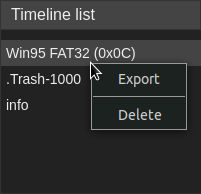
\includegraphics[width=4.5cm]
	{./figures/timeline-list.png}
	\centering
	\caption{Img-spy timeline list}
	\label{F:img-spy-timeline-list}
\end{wrapfigure}

The generation of timelines is computed on parallel using a child of electron's
main process. Some items are received with short periods of time. Instead of 
delivering one action each time an item is received, in order to reduce
unnecessary fast renderings, timeline results are buffered and delivered each
100ms at most.

\subsubsection{Timeline list}

Timeline list (Figure \ref{F:img-spy-timeline-list}) contains all generated
timelines. When its generation is finished, the data of the timeline is stored
on the current case settings and thus auto-saved.

Each item of the list has a context menu export a timeline using CSV format.
The other button is used remove the timeline item from the list and settings.

\subsubsection{Timeline table}

The timeline table (Figure \ref{F:img-spy-timeline-table}) contains the results
of a specific timeline. The user can order columns clicking the headers and 
move to different pages using previous and next buttons.

\begin{figure}[htb]
	\begin{center}
		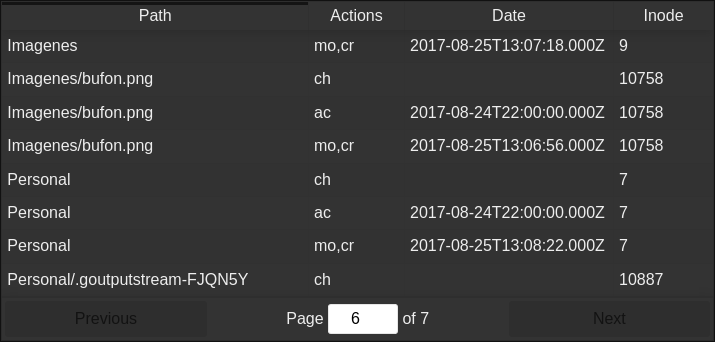
\includegraphics[width=0.8\textwidth]
		{./figures/timeline-table.png}
		\caption{Img-spy timeline table}
		\label{F:img-spy-timeline-table}
	\end{center}
\end{figure}

The fist column is the item path and the second one are the two first letters of
the actions (created, modified, changed and accessed). Then the date of the 
action, and the last is the inode.

\subsection{Search}

Finally, \textit{Search} uses tsk-js search functionality to let the
user look for a string inside the image. This execution is executed in parallel
and when all results are retrieved, they are saved on settings, as
\textit{Timeline} (see Chapter \ref{S:timeline}).

\subsubsection{Search from}

\begin{wrapfigure}[10]{L}{5.5cm}
	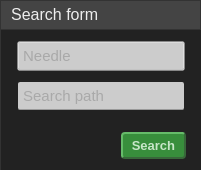
\includegraphics[width=5cm]
	{./figures/search-form.png}
	\centering
	\caption{Img-spy search form}
	\label{F:img-spy-search-form}
\end{wrapfigure}

Search form (Figure \ref{F:img-spy-search-form}) has two inputs: needle and
search path.

\begin{description}
	\item[Needle] Text that will be looked inside the image.
	\item[Search path] This field is not editable. It has the path of the
	selected item on case structure (Chapter \ref{S:case-structure}).
\end{description}

When user clicks search button, the search process starts to look for matches
on background and each time a result is retrieved, it appears on the search
result's table.

\subsubsection{Search list}

\begin{wrapfigure}[9]{R}{6cm}
	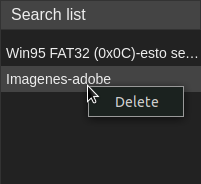
\includegraphics[width=5cm]
	{./figures/search-list.png}
	\centering
	\caption{Img-spy search list}
	\label{F:img-spy-search-list}
\end{wrapfigure}

All queried search appears on search list (Figure
\ref{F:img-spy-search-list}). When the look up finishes, it is stored on the
current case settings and thus auto-saved.

Each item of the list has a context menu with the option to delete this item
from the list and settings.

\subsubsection{Search results}

The results of the selected search item are displayed on a table inside this
panel (Figure \ref{F:img-spy-search-results}). This table, as \textit{Timeline}
table, also supports custom order by clicking the headers.

The first column shows the path of the files that contains the needle and 
how many times it appears. If the toggle button is clicked, the row
uncollapses and shows the context and index where the string if appears inside
this file.

\begin{figure}[htb]
	\begin{center}
		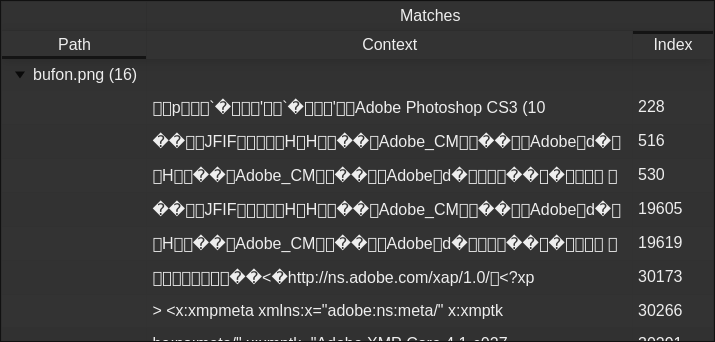
\includegraphics[width=0.8\textwidth]
		{./figures/search-results.png}
		\caption{Img-spy search results}
		\label{F:img-spy-search-results}
	\end{center}
\end{figure}

\section{Key developments}

There were many difficult or interesting parts on the development of this 
project. Some of them are multiple themes support, file system watcher, 
auto-save settings, tsk-js workers and resize panels. Also, some plug-ins where
used to increase the development speed.

\subsection{Multiple themes support}

When designing user interfaces, colors are very important. A good consideration
is to take profit of SASS define palettes and work with them. That way, to
support multiple themes is as easy select some palettes to work. The palette
format used is the one defined by Google Materials \cite{google-materials-web}.
Each theme has:

\begin{description}
	\item[Main palette] Is used for the main layout.
	\item[Primary palette] Define colors for components that must be
	highlighted.
	\item[Warn palette] Notifies the user that something is wrong. Red palette
	is normally used.
	\item[Background] Default background color.
	\item[Foreground] Default foreground color.
\end{description}


\subsection{File system watcher}

A React component has been created to launch redux actions notifying file
system changes. It uses Node.js package \textit{"chokidar"} to watch those
changes efficiently. Watcher is bound using \textit{"componentWillMount"}
lifecycle function.

Then, several Redux-Observables epics chain actions, such as, launch tsk-js
analysis function if the payload contains an image.

\subsection{Auto-save settings}

To implement the auto-save functionality, some epics actions map to update
settings model action. The auto-save epic (Listing \ref{L:auto-save-epic})
launch another to save them inside the user's disk.

\begin{codefigure}
	\tsexternal[
		classoffset=1,
		morekeywords={EpicObservable, ImgSpyState},
		%
		caption=Mapping example,
		label=L:auto-save-epic,
	]{source/auto-save.epic.ts}
\end{codefigure}

\subsection{The Sleuth Kit JavaScript workers}

As explained before, JavaScript doesn't support multithreading (Chapter
\ref{S:electron}). To do not freeze any Electron process while performing
tsk-js tasks, main process launch four subprocesses.

Those subprocesses act as workers. Each time a task is received, if any worker
is free, it takes this tasks and execute it. If none is free, the task is 
queued.

\subsection{Resize-panels}

An other React component was created to perform the resizing of panels. This
component launch a resize-start Redux action when the slider is mouse down, a
resize when the user moves the mouse and a resize-stop when the mouse is 
released.

Each time those actions are received, the resize-panel refresh its children
size using CSS properties.

\subsection{React plug-ins}

All the application forms uses \textit{react-redux-form} package. It provides
React components that store the form model inside the redux state. In this
manner, the form values are accessible from any other React component.

Timeline and Search result tables are drawn using \textit{react-tables}. This 
package has React components to render tables very fast. Those tables have 
order by, pagination and row aggregation functionalities implemented.

\section{Code quality analysis}

% TODO: No se si es interesante poner esto aunque creo que da una idea de como
% esta hecho si crees que esta bien explico cada valor si esta bien o que 
% se puede mejorar

To check if the project is scalable enough, some code quality metrics are 
calculated. The command used is \textit{sloc}.


\begin{terminal}[
	caption=Code quality CSV extraction using sloc,
	label=L:sloc-code-quality
]
%
\terminalcmd[sloc -d -f csv -e lib src/ > code-quality.csv]
%
%\terminalcmd%

\end{terminal}

With this information, some interesting metrics can be computed. Table

\begin{table}[htb]
\begin{center}
\begin{tabular}{|l|l|l|}
\hline
{\bf Metric }	& {\bf Value} & {\bf Expected} \\ \hline \hline
Total files & 190 & - \\ \hline
Source lines & 8779 & - \\ \hline
\hline

Max. source lines per file & 301 & \textless\space\text{300} \\ \hline
Min. source lines per file & 1 & \textgreater\space\text{1} \\ \hline
Avg. source lines per file & \approxtext\text{46} & \textless\space\text{100} \\ \hline
\hline
Files without comments & 70.5\% & \textless\space\text{20\%} \\ \hline
Comments / Source & 2\% & \textgreater\space\text{5\%} \\ \hline
Avg. code blocks size & 4 & - \\ \hline
\end{tabular}
\caption{Code analysis metrics}
\label{T:code-analysis-metrics}
\end{center}
\end{table}






